


\section{Classification}
\subsection{The problem}
We chose to look at classifying by state, as that was one of the few nominal attributes in our data set. We also considered computing a new attribute corresponding to the dominant ethnicity of the community population. However, we are sceptical that any meaningful classification can be made.

\subsection{Model application}
Our naive bayes implementation yielded an error rate of 73.17\% for our dataset using k=10 for the k-fold crossvalidation.
    \begin{figure}[H]
      \centering
        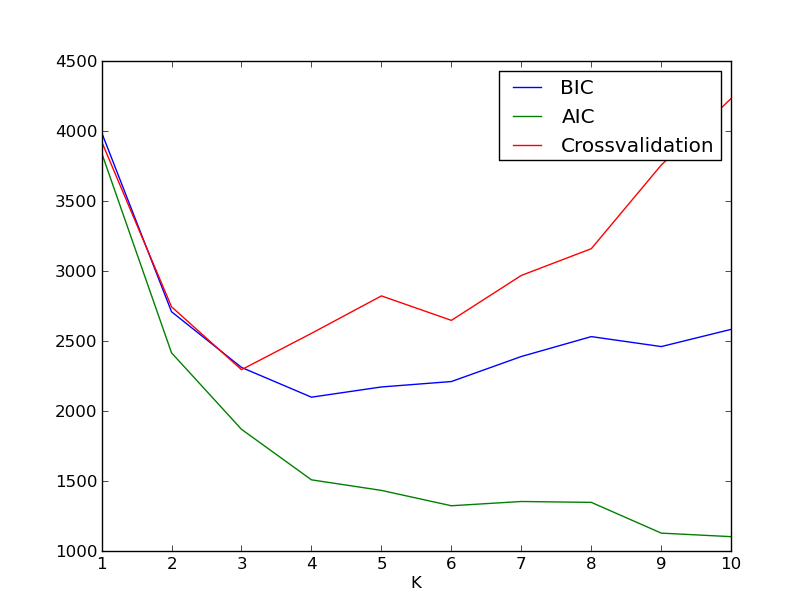
\includegraphics[width=0.7\linewidth]{figures/figure_2}
        \caption{Error rates for Naive Bayes.}
        \label{fig:k}
    \end{figure}

Our K-nearest neighbours implementation (run with maximum neigbours 30 and only on a subset of our attributes due to time constraints) gave the following error rates
    \begin{figure}[H]
      \centering
        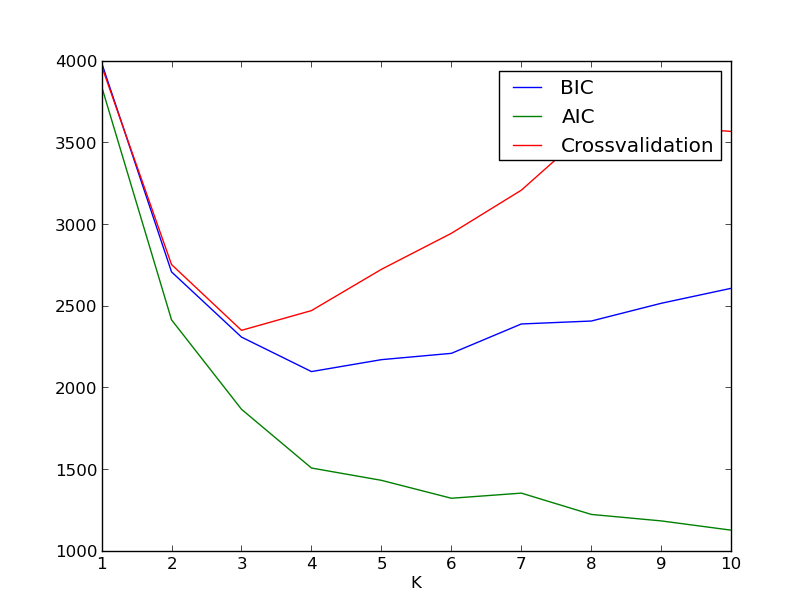
\includegraphics[width=0.7\linewidth]{figures/figure_1}
        \caption{Error rates for K-nearest neighbours.}
        \label{fig:k}
    \end{figure}

\subsection{Classification of new data}
New data may be predicted using the the knclassifier object of the prefered model. Similarly, the nb\_classifier may be used for the Naive Bayes model.

For the K-nearest neighbours model, new data is classified by taking the majority class of the k nearest neighbours.

The error rates look very suspicious, probably due to either programming error or that the data doesn't classify easily.

\subsection{T-test}
    \begin{figure}[H]
      \centering
        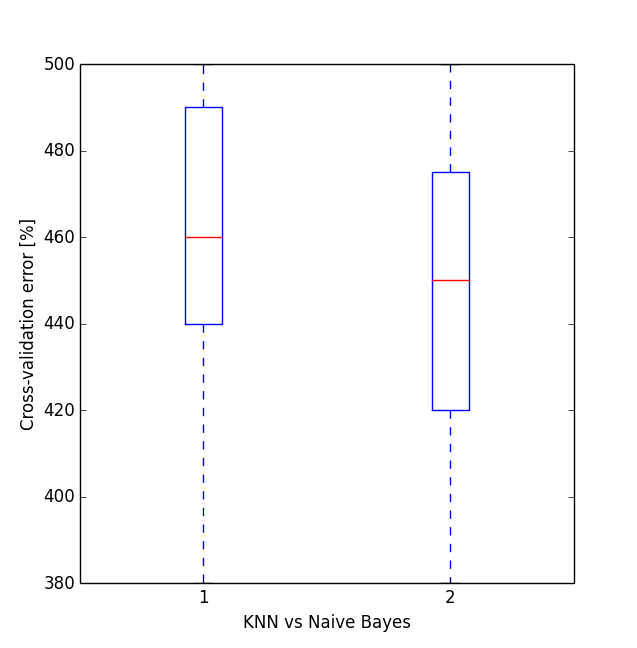
\includegraphics[width=0.7\linewidth]{figures/knnvsnaive}
        \caption{T test of KNN and Naive bayes.}
        \label{fig:k}
    \end{figure}
    \begin{figure}[H]
      \centering
        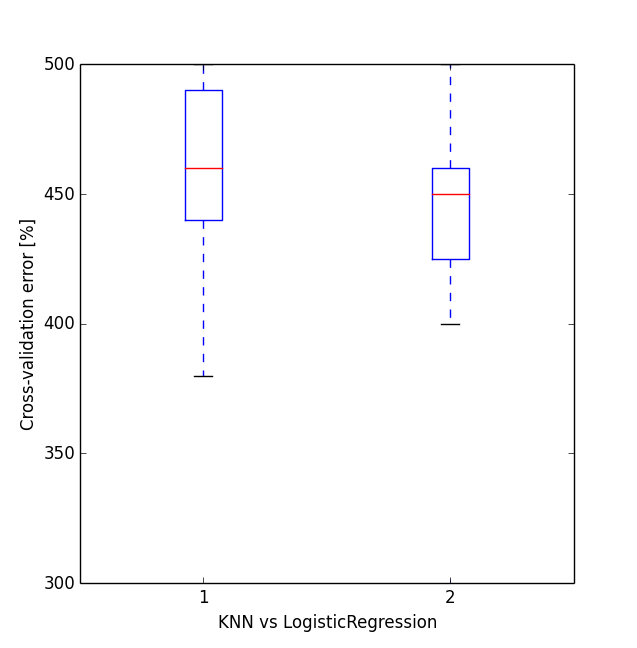
\includegraphics[width=0.7\linewidth]{figures/knnvslog}
        \caption{T test of KNN and Logistic Regression.}
        \label{fig:k}
    \end{figure}
    \begin{figure}[H]
      \centering
        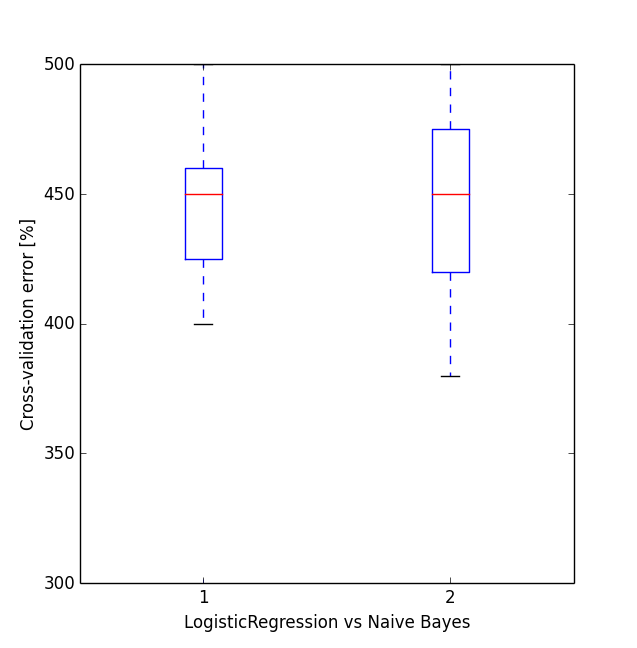
\includegraphics[width=0.7\linewidth]{figures/logvsnaive}
        \caption{T test of logistic regression and Naive bayes.}
        \label{fig:k}
    \end{figure}
Our t-test yields that the k-nearest neighbour and naive bayes classifier models are significantly different (with p=0.0007135281700851776). The other t-test comparisons gave us that the models weren't significantly different.

